\documentclass[tikz,border=7pt]{standalone}
\usepackage{amsmath}
\usetikzlibrary{arrows.meta,positioning,fit}

\tikzset{
  comp/.style={
    draw,rectangle,rounded corners=2pt,
    minimum width=34mm,minimum height=24mm,align=center
  },
  conn/.style={-{Latex[length=2.1mm]},thick}
}

\begin{document}
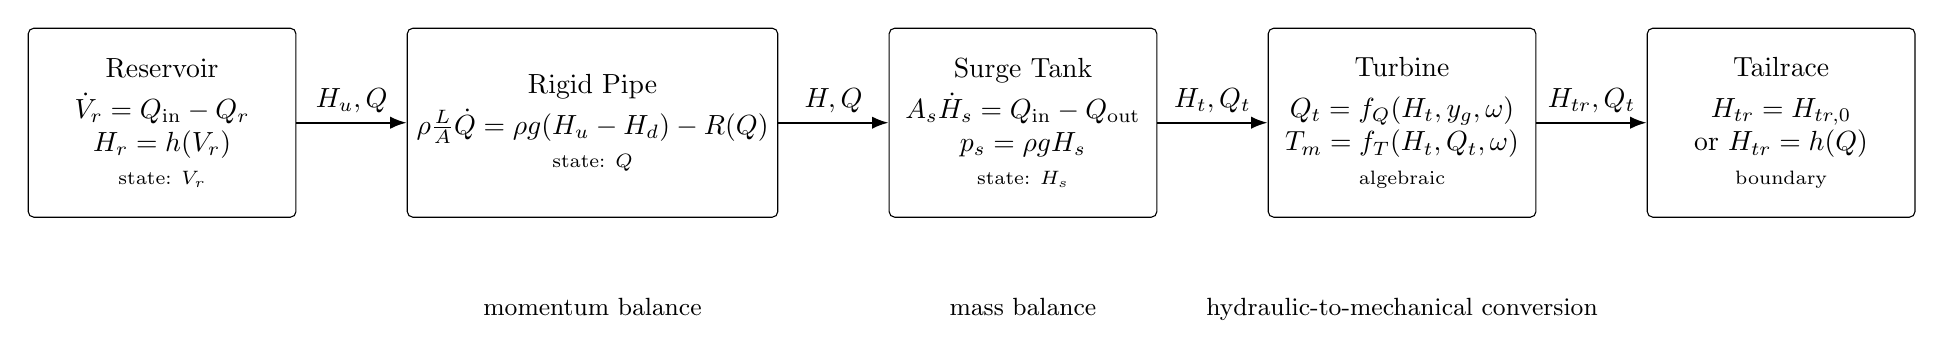
\begin{tikzpicture}[node distance=14mm]

\node[comp] (res) {
Reservoir\\[1mm]
$\dot V_r = Q_{\mathrm{in}}-Q_r$\\
$H_r = h(V_r)$\\
\scriptsize state: $V_r$
};

\node[comp,right=of res] (pipe) {
Rigid Pipe\\[1mm]
$\rho \frac{L}{A}\dot Q =
\rho g(H_u-H_d)-R(Q)$\\
\scriptsize state: $Q$
};

\node[comp,right=of pipe] (surge) {
Surge Tank\\[1mm]
$A_s\dot H_s = Q_{\mathrm{in}}-Q_{\mathrm{out}}$\\
$p_s=\rho g H_s$\\
\scriptsize state: $H_s$
};

\node[comp,right=of surge] (turb) {
Turbine\\[1mm]
$Q_t=f_Q(H_t,y_g,\omega)$\\
$T_m=f_T(H_t,Q_t,\omega)$\\
\scriptsize algebraic
};

\node[comp,right=of turb] (tail) {
Tailrace\\[1mm]
$H_{tr}=H_{tr,0}$\\
or $H_{tr}=h(Q)$\\
\scriptsize boundary
};

\draw[conn] (res) -- node[above] {$H_u,Q$} (pipe);
\draw[conn] (pipe) -- node[above] {$H,Q$} (surge);
\draw[conn] (surge) -- node[above] {$H_t,Q_t$} (turb);
\draw[conn] (turb) -- node[above] {$H_{tr},Q_t$} (tail);

\node[below=9mm of pipe,align=center] {\small momentum balance};
\node[below=9mm of surge,align=center] {\small mass balance};
\node[below=9mm of turb,align=center] {\small hydraulic-to-mechanical conversion};

\end{tikzpicture}
\end{document}
